\subsection{Distributed approach with communication}
\label{subsec:ex1comm}


\subsubsection{Model training}
\label{subsubsec:learnedcomm}

Using the same dataset collected using the expert controller to perform the task 
without communication, it is possible to train a ``distributed network with 
communication'' that at each timestep takes as input for each robot an array 
containing the response values of the sensors – which can be either 
\texttt{prox\_values}, \texttt{prox\_comm} or \texttt{all\_sensors} – and the 
message received in the previous timestep, communicated by the nearest agents 
(one on the left and one on the right), and produces as output an array of 2 
floats, corresponding the first one to the control, that as before is the speed of the 
wheels, and the second one to the communication, i.e. the message transmitted 
by the robot to the nearest agents.

As before, the model is independent of the number of agents in the simulations, 
instead, in this approach is important to keep track of the timesteps order since 
the input of the network requires the communication received, that corresponds 
to a message transmitted in the previous timestep. 
To do so, a preprocessing is applied to the dataset in order to combine 
consecutive timesteps into a set of sequences. Therefore, we divide each 
simulation in sequences of length $2$, or composed by two consecutive 
timesteps, using a stride of $1$ among them, that contains an ordered series of 
two states for each robot.   

In this case, the input shape is transformed from $1 \times \mathtt{input\_size}$ 
to $\mathtt{seq\_length} \times N \times \mathtt{input\_size}$, where 
\texttt{seq\_length} is fixed at $2$, while $N$ is variable and \texttt{input\_size} 
can be $7$ or $14$.

\begin{figure}[htb]
	\centering
	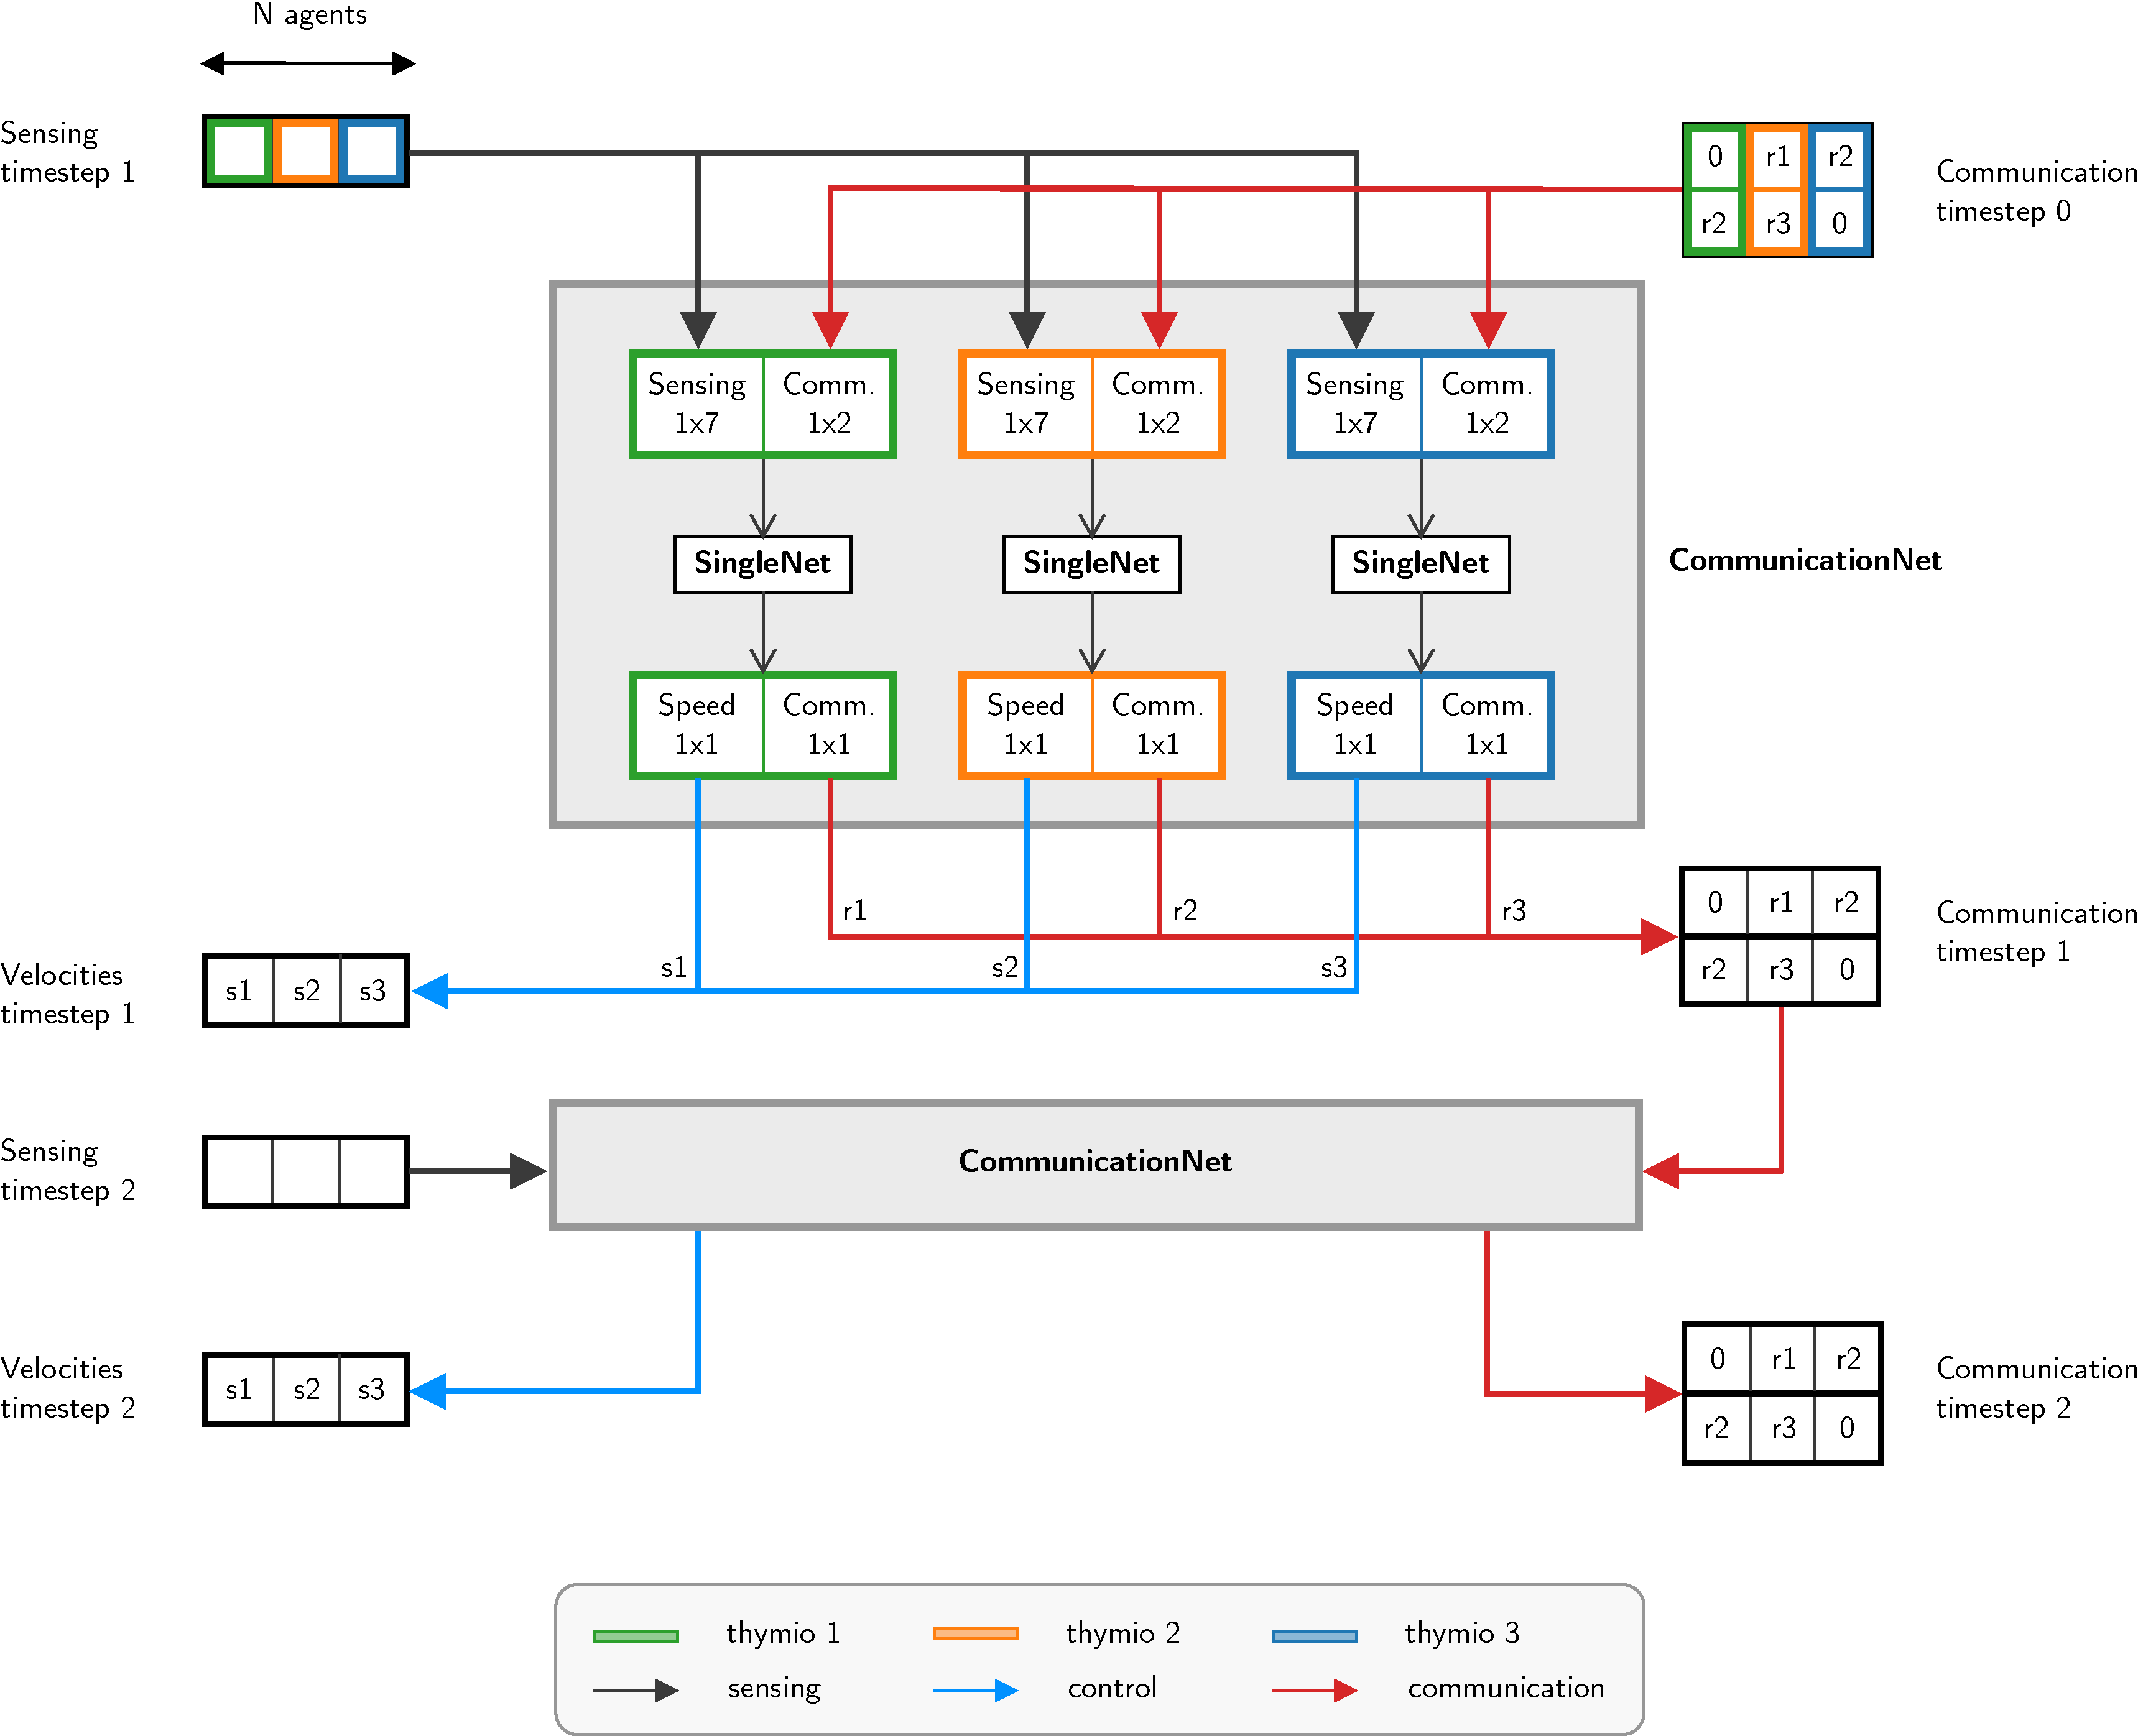
\includegraphics[width=\textwidth]{contents/images/commnet}
	\caption[Communication network.]{Visualisation of the forward pass of the 
	communication network with three agents and a sequence composed by two 
	timesteps.}
	\label{fig:commnet1}
\end{figure}

It is important to notice that the communication is not yet in the input since it is 
not contained in the dataset, instead is treated as a hidden variable to be inferred. 
In particular, since in the first timestep no messages have been received yet, we 
initialise randomly a placeholder, that has the dimension of the number of agents 
plus two, using float values in the range $[0, 1]$. 
Moreover, the communication value for the first and last agents would always be 
$0$, since we want to distinguish the fact that the two extreme robots never 
receive messages respectively from the left or from the right.
For this reason, we define a recurrent structure of the communication network, 
shown in Figure \ref{fig:commnet1}, composed by two nested modules: in the 
high-level operates the \texttt{CommNet} that handle the sensing of all the 
agents, while in the low-level \texttt{SingleNet} that works on the sensing and the 
communication received by a single agent in a certain timestep, producing as 
output the control and the communication to transmit. 

The architecture of the \texttt{SingleNet}, displayed in Figure 
\ref{fig:singlenetcomm1}, is almost the same as the one of the distributed model 
without communication: there are three linear layers each of size 
$\langle\mathtt{input\_size} + 2, 10\rangle$,  $\langle 10, 
10\rangle$ and $\langle 10, 2\rangle$, where \texttt{input\_size} is the sum of 
the shape of the sensing and the two communication values received, one from 
the left and one from the right.

\begin{figure}[H]
	\centering
	\begin{subfigure}[h]{0.495\textwidth}
		\centering
		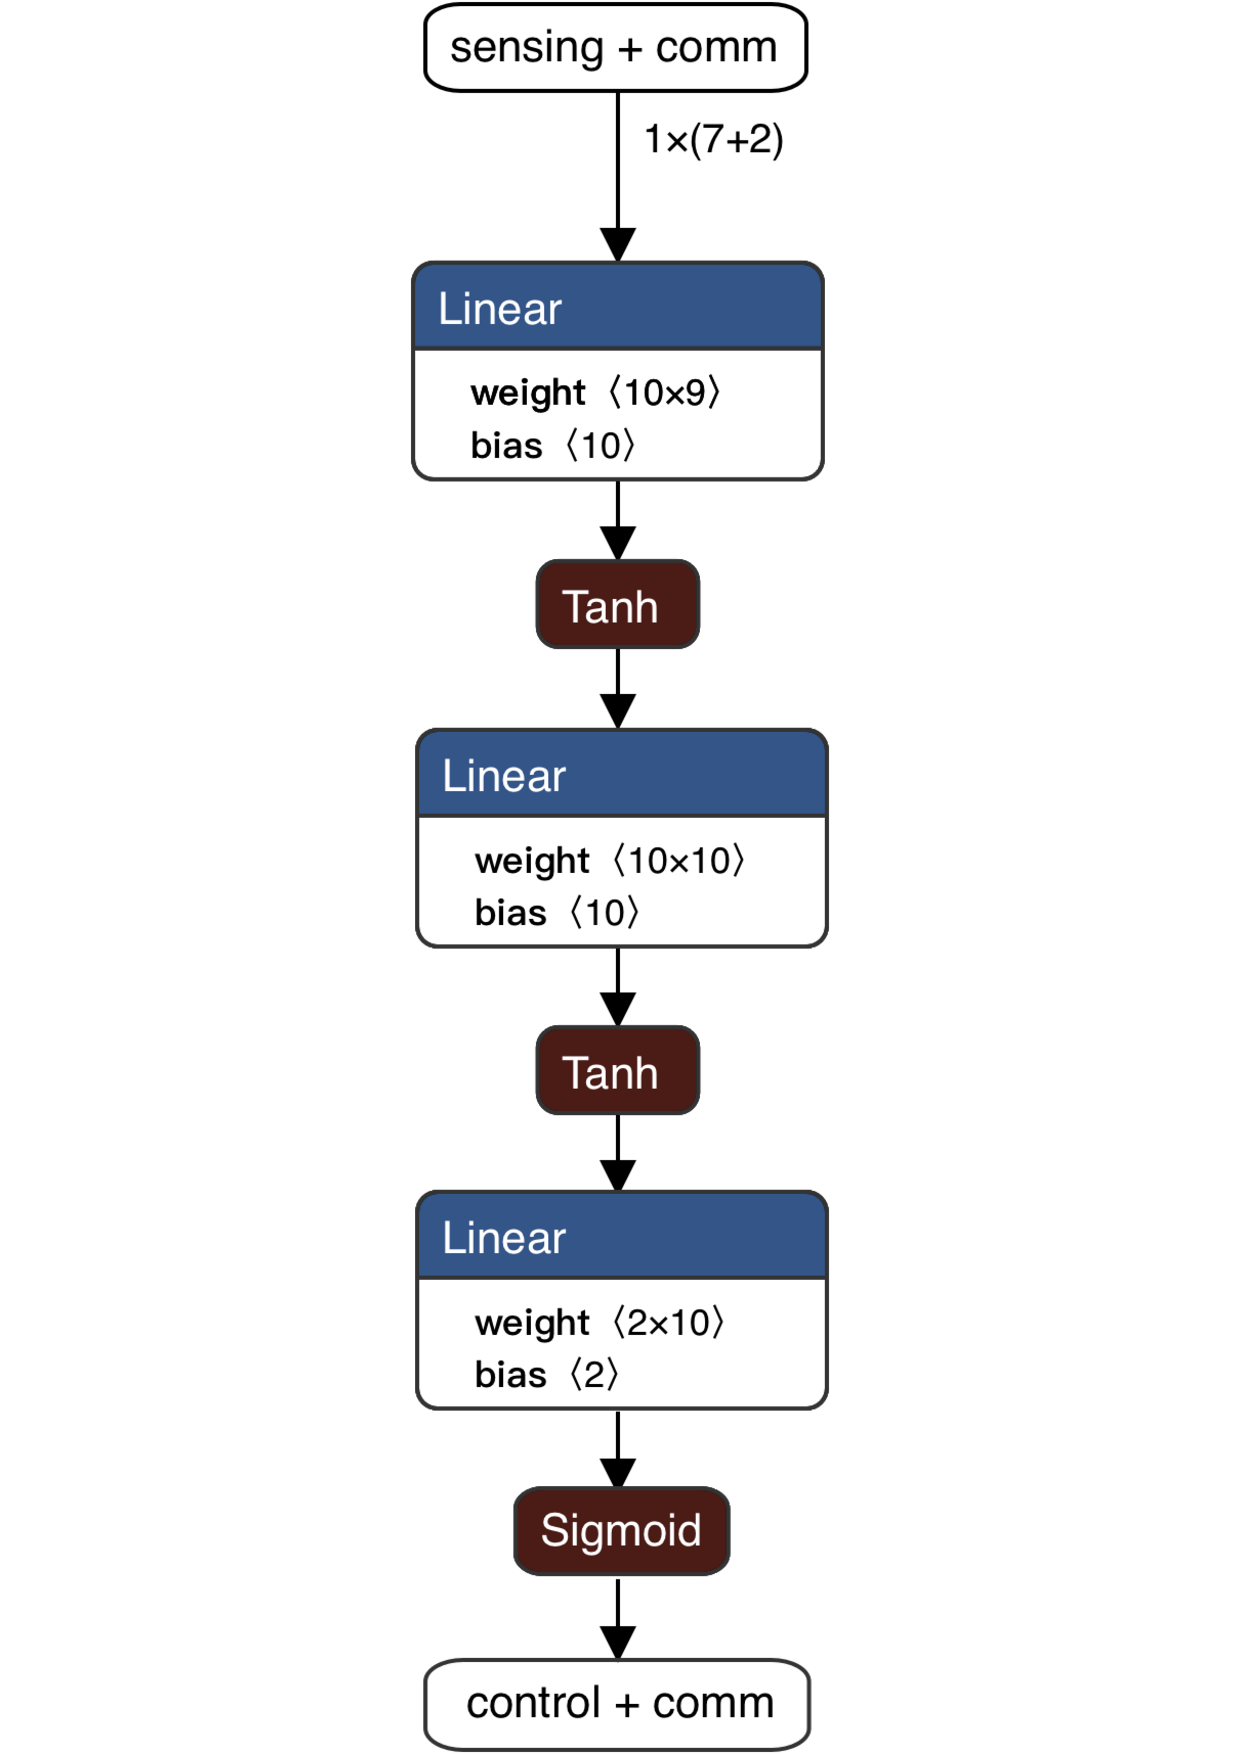
\includegraphics[width=.3\textwidth]{contents/images/task1distributedcomm@4x}%
		\caption{Structure of the \texttt{SingleNet} with communication and $7$ 
		input sensing.}
	\end{subfigure}
	\hfill
	\begin{subfigure}[h]{0.495\textwidth}
		\centering
		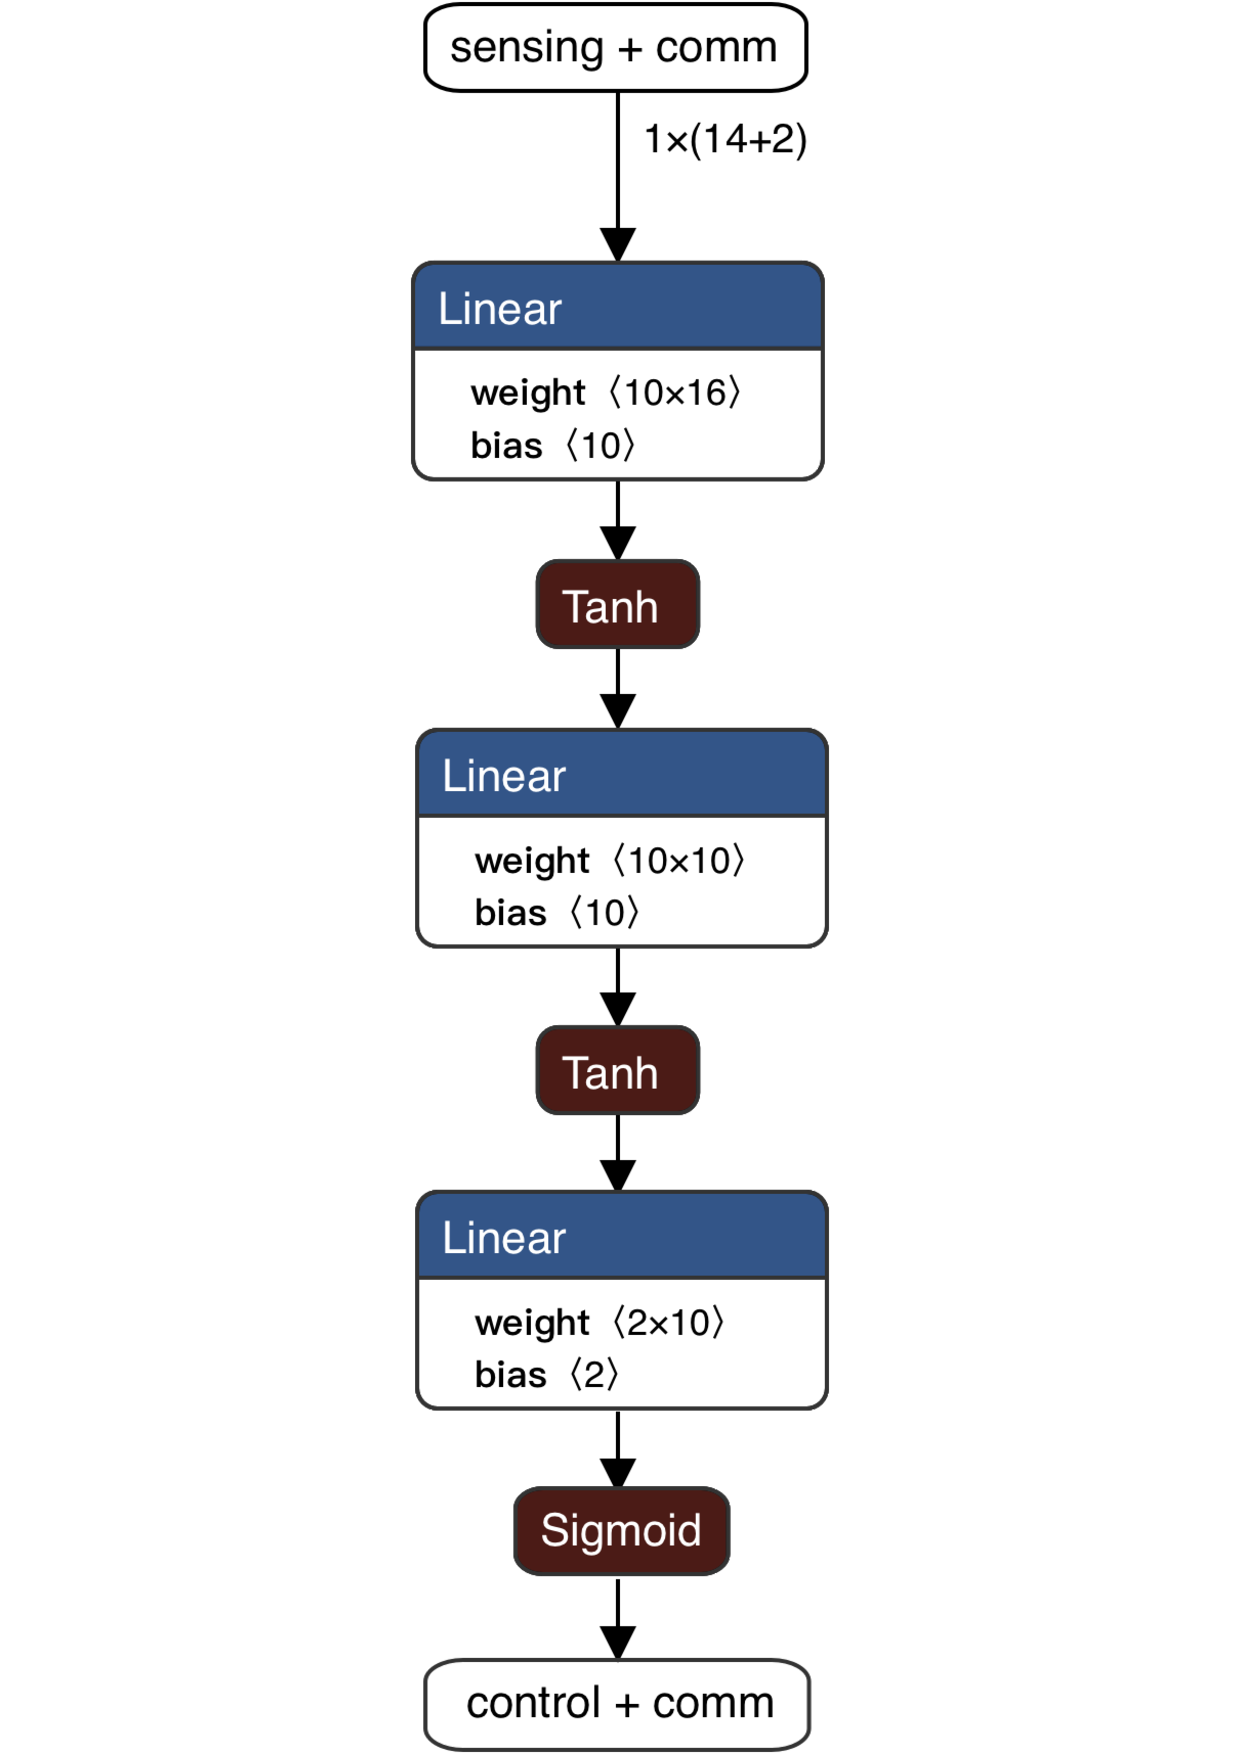
\includegraphics[width=.3\textwidth]{contents/images/task1distributed_allcomm@4x}
		\caption{Structure of the \texttt{SingleNet} with communication and $14$ 
		input sensing.}
		\label{fig:singlenet14comm1}
	\end{subfigure}
	\caption[Network architectures for the distributed approach with 
	communication.]{Visualisation of the network architectures for the distributed 
	approach with communication.}
	\label{fig:singlenetcomm1}
\end{figure}

As before, to the first and second layer is applied a tanh non-linear activation 
function, while a sigmoid \cite[see][]{han1995influence}, shown in Figure 
\ref{fig:sigmoid}, is applied to the second dimension of the output, that is the 
value of the communication to transmit, in order to normalise it in the range $[0, 
1]$ and its output is given by
\begin{Equation}[htb]
	\centering
	\begin{equation}
	\sigma(x)= \frac{1}{1 + e - x}
	\end{equation}
	\caption{Sigmoid Function.}
	\label{eq:sigmoid}
\end{Equation}

\noindent
Since applying this activation function the message to be transmitted is a float 
between $0$ and $1$, it will be later transformed into an integer and rescaled 
between $0$ and $1023$ so that it is in the format expected by the Thymio.

\begin{figure}[htb]
	\centering
	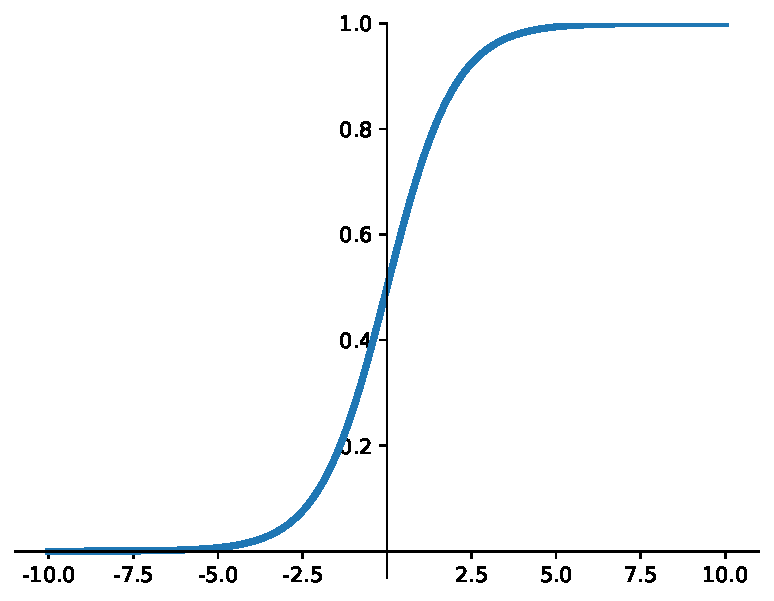
\includegraphics[width=.5\textwidth]{contents/images/sigmoid2}%
	\caption{Trend of the Sigmoid activation function.}
	\label{fig:sigmoid}
\end{figure}

As before, we use Adam optimiser but with a smaller learning rate, $0.001$. We 
split the dataset in mini-batches, this time of size $10$ and then train the models 
for $500$ epochs. 

Finally we evaluate the goodness of the predicted control using the \gls{mse} loss 
function, while the communication is learned in an unsupervised way.
Since the network is fully connected, the communication affects directly the 
output, and consequently, the error minimised, even if it is computed using only 
the control. Improving the loss have an impact also on the communication latent 
variable: since the error is propagated through the internal network, in order to 
update the weight during the back-propagation step, that affects the 
communication.

\subsubsection{Experiments}
\label{subsubsec:expcomm}
